\section{Motivation}
Often, in a problem being tackled with Machine Learning (ML) techniques, one of the most important parts of the solving process is the algorithm selection. Each algorithm has a specific bias, making it more suitable for some classes of problems than others \cite{Adam2019}. It is desirable, then, that we may have a way of measuring the relationship of the performance of a given algorithm in a problem with the problem's characteristics since knowing which data is easy or difficult for a given model to classify is useful in the way that we may make changes to the original model.

\citeonline{Munoz2018} has introduced a methodology called Instance Space Analysis (ISA), a novel way of performance evaluation and algorithm selection in classification problems by mapping the statistical properties of an instance (an entire dataset) into how difficult the instance is for a set of classification algorithms to perform. Further, in \citeonline{Lorena2022}, the methodology has been modified to have a more fine-grained analysis, with the instance being reduced to an individual observation in a classification dataset.

Given this, we can map each observation to a hardness level. However, one feature of the ISA not investigated in the instance-level proposal of \citeonline{Lorena2022} is how to generate new instances with desired characteristics to expand the dataset with observations that may defy the classification techniques at different levels. This project aims to fill this gap. 

One type of model that may give us this feature from this data is a neural network that encodes the data into the instance space and decodes from it. Using this approach, we can then generate data in a target region of the instance space and use the decoding part of the network to infer a reconstruction of the original data and find difficulty metrics from it, as well as be able to challenge the classification techniques at different levels. We can use this to verify how the original model behaves with data with a given instance space profile or to challenge the model, such as generating adversarial examples \cite{Yuan2019}.
%a Generative Adversarial Network (GAN) architecture, as defined by \citeonline{Goodfellow2014}. This architecture is based on a zero-sum game, with a generator network trying to create data matching the original data and a discriminator network trying to discern between the original data and the generated data. 
%
%Using this approach, we can use the trained generator to create data with specific hardness levels and be able to challenge the classification techniques at different levels. We can use this to verify how the original model behaves with data with a given difficulty profile or to challenge the model, such as generating adversarial examples \cite{Yuan2019}.

\section{Objective}

This work aims to provide a framework for data generation based on the instance space generated for a dataset. Therefore, new data instances can be generated for target regions of the instance space. Next, we monitor the original model's behavior using the generated data.

\section{Scope}

The scope of this work will be limited to exploring an encoder-decoder implementation for the generation of data.  The modelling will be made entirely using Python, with the PyTorch \cite{paszke2019pytorch} framework. PyHard \cite{Lorena2022} will be used for reproducing the ISA methodology.

%\begin{figure}[ht]
%\centering
%
\includegraphics[width=0.5\textwidth]{Cap1/cupim}
%\caption{Proibido estacionar cupins. Legenda grande, com o objetivo de demonstrar a indentação na lista de figuras.}
%\label{cupim}
%\end{figure}


%\begin{figure}[ht!]
%\centering
%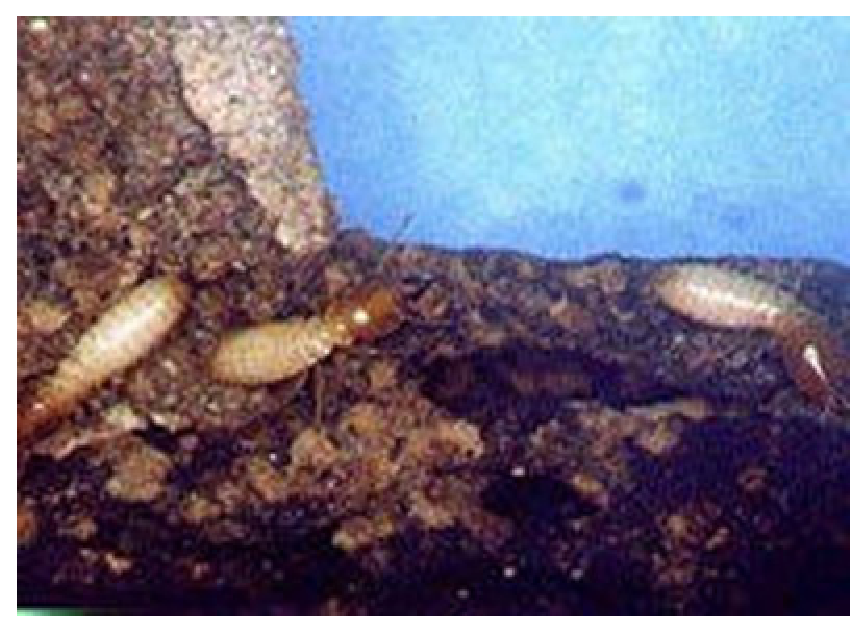
\includegraphics[width=1\textwidth]{Cap1/cupimconcreto}
%\caption{Exemplo real de cupim frente ao seu dilema.}
%\label{FDII}
%\end{figure}

\section{Outline of this work}

The document is organized as follows:

\begin{itemize}
	\item Chapter \ref{ch:machinelearning}  introduces some Machine Learning terminology and describes the encoder and decoder neural network models;
	\item Chapter \ref{ch:isa} describes the ISA framework;
	\item Chapter \ref{ch:methodology} presents the methodology to be followed in the computational experiments;
    \item Chapter \ref{ch:results} shows the results of the application of the methodology;
	\item Chapter \ref{ch:conclusion} concludes the work.% presenting future activities and a work schedule.
\end{itemize}
